\section{Brugervejledning til ReflexBall}
Spillet Reflexball er et arkanoid spil, som handler om at ramme kasser med en bold. Bolden skal holdes i live med en striker, som reflekterer bolden op mod kasserne. Hvis bolden ikke rammer strikeren, og dermed ryger ud af banen, mister man et liv. Kasserne har forskellig styrke alt efter hvilken farve de er. Styrken svarer til det antal gange kassen skal rammes, før den bliver ødelagt. Her er en liste, hvor styrken står til venstre og farven til højre.
\begin{enumerate}
\item Lyseblå
\item Lilla
\item Blå
\item Pink
\item Grøn
\end{enumerate}

Når brugeren starter spillet vises en menu. Her kan brugeren styre markøren med knapperne til venstre og i midten. Brugeren vælger den mulighed som markøren står foran ved brug af den højre knap. I menuen kan brugeren se instruktioner, og vælge sværhedsgrad. Når brugeren vælger at starte spillet, vil spillet loade, og bolden sættes over strikeren. Brugeren flytter strikeren ved brug af den venstre og midterste knap. Når brugeren ønsker at sætte bolden i gang trykkes på knappen til højre. Når spillet er i gang kan spillet sættes på pause ved at trykke på den højre knap, og spillet startes da igen ved et tryk på højre knap. Hvis brugeren mister alle sine liv, afsluttes spillet og vender tilbage til menuen. Hvis spilleren derimod får ødelagt alle kasserne vil næste level loade. Ved det sidste level vil en victory screen loade, og vende tilbage til menuen. \\
\begin{figure}[h]
\begin{center}
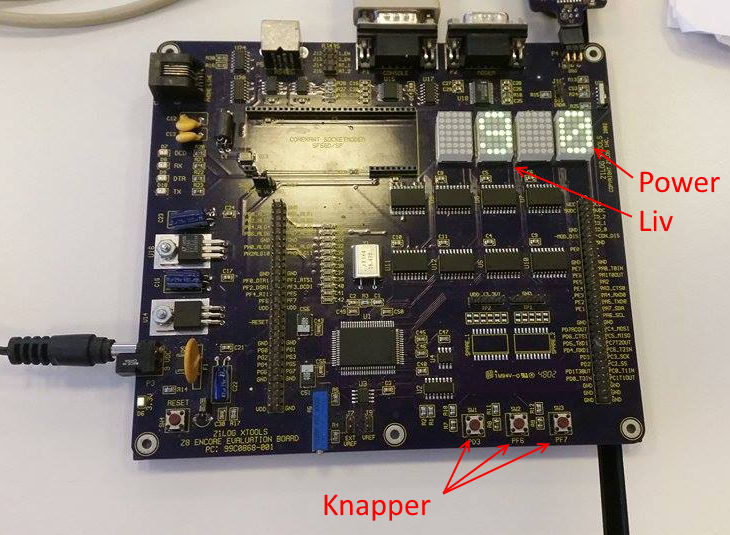
\includegraphics[scale=0.6]{img/Board.png}
\end{center}
\end{figure}
Spillets sværhedsgrad har indflydelse på, hvor hurtigt bolden bevæger sig, og hvor mange liv man har. Når man spillet på easy har brugeren 9 liv, og bolden bevæger sig forholdsvis langsomt. På medium er antallet af liv 5, og farten er sat lidt op. På hard har brugeren 3 liv og farten er høj.
\\
Bolden har også egenskaben High Power. Egenskaben aktiveres ved at trykke på den venstre og den midterste knap samtidigt.  For hver kasse som brugeren ødelægger, bliver power 1 større. Power skal være 5, før brugeren kan aktivere High Power. Når High Power er aktiveret ødelægger bolden kasserne uanset hvilken holdbarhed de har. Dog mister man 1 power for hver kasse man ødelægger. High Power bliver deaktiveret igen når power er 0. Power  bliver nulstillet hvis man mister et liv. Man kan maksimalt have et Power niveau på 9, derefter tæller den ikke yderligere op. \\

Der findes en hemmelig feature: En boss key er implementeret, som sletter alt hvad der er på skærmen. Denne tilstand aktiveres ved at trykke på alle tre knapper på samme tid. Tilstanden er dog permanent, og spillet skal genstartes, hvis man fortsat vil spille, når chefen er gået. 
